% ------------ F/h2  ------
\section{F-h$^2$ analysis}
The analysis of $F$ vs $h^2$  follows \cite{mcgurk1999,Malzbender200172,Malzbender2000265}.

\begin{figure}[h]
  \centering
  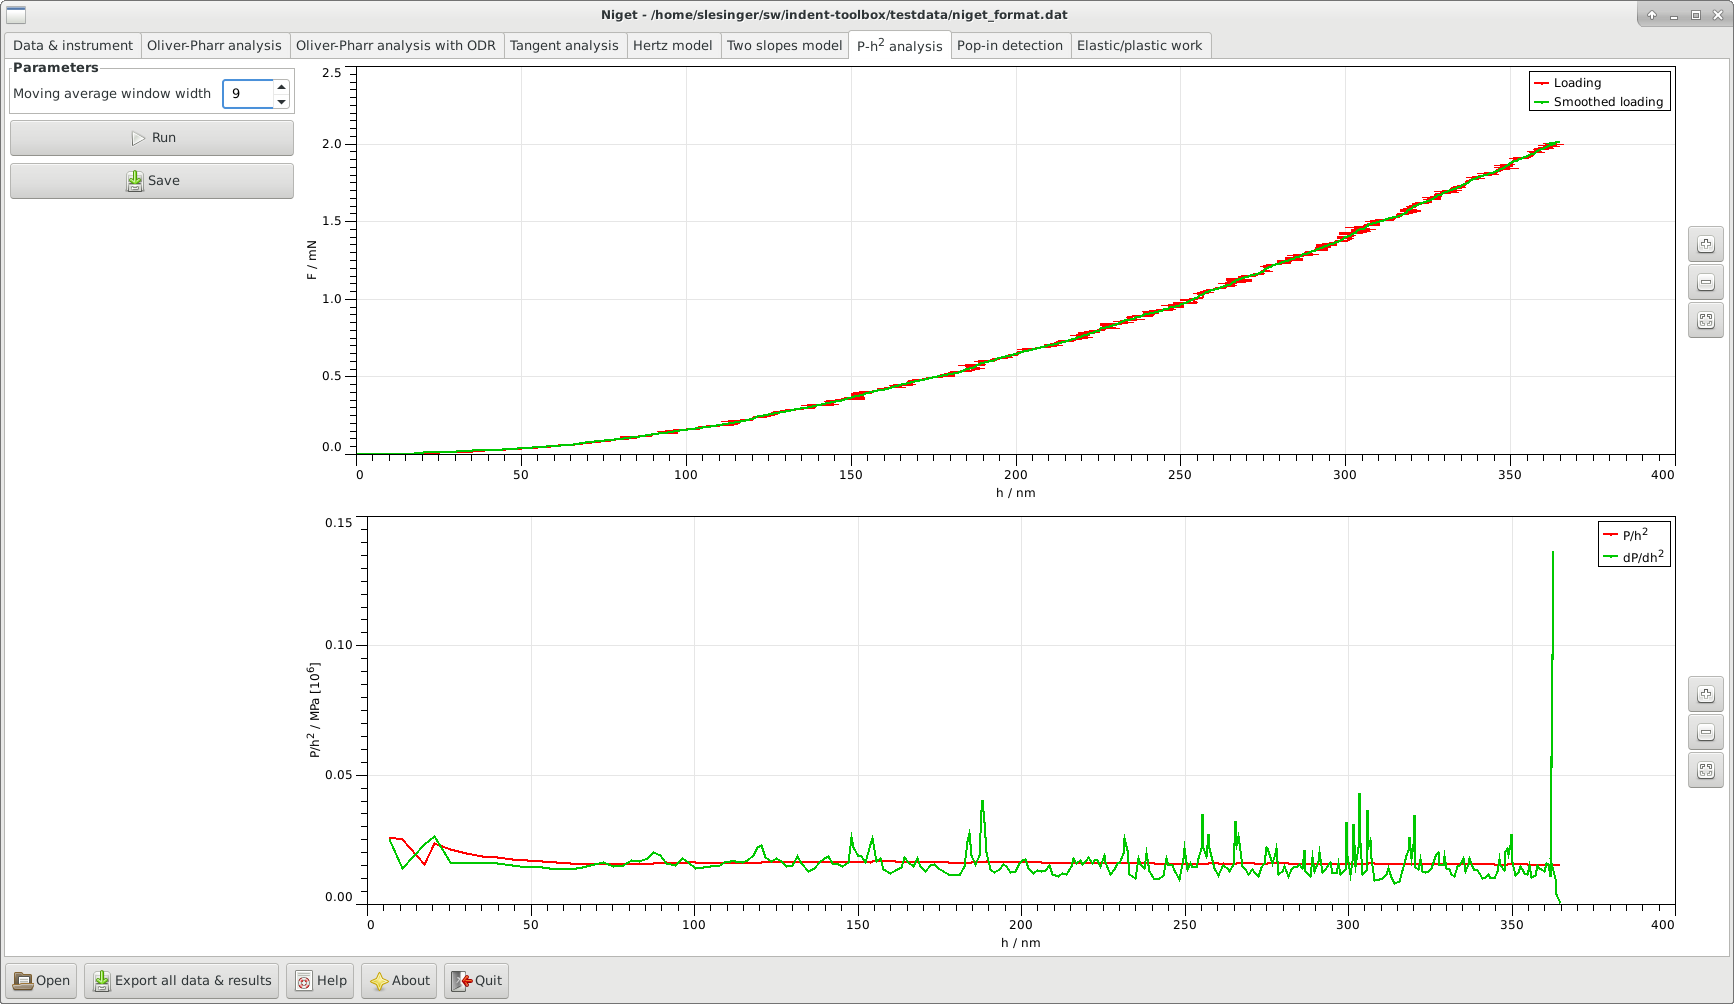
\includegraphics[width=\textwidth]{images/screen-ph2}
  \caption{$F$ vs $h^2$ analysis}
\end{figure}

\subsection{Window}
The window consists of several blocks:
\begin{itemize}
 \item \emph{Parameters} allows the user to set the width of the moving average window. The value~1 corresponds to no smoothing. This value is saved in settings. 
 \item \emph{Run}  perform calculation and display curve, see section \ref{Ph2_calc}. 
 \item \emph{Save} save parameters and results to given file. 
 \item \emph{Graph}  
    \begin{itemize} \item[] Top: display the loading curve and the smoothed curve. 
		    \item[] Bottom: display the $F/h^2$ and the $\mathrm{d}F/\mathrm{d} h^2$ curves.     
    \end{itemize}
 Stepwise zooming/unzooming can be performed by selecting a range with the mouse and pressing the \emph{Zoom}/ \emph{Unzoom} buttons. 
		     The graph is restored to its original size by the \emph{Restore} button. Zooming in the two graphs is independent.
  \end{itemize}

\subsection{Procedure}\label{Ph2_calc}
\begin{enumerate}
 \item 
We use a moving average with a fixed width and constant weight. This means we substitute a value with its average with $s$ values to the left and to the right, $w = 2s + 1$ 
$$
\hat{x} _i = \frac1w \sum_{j = -s}^{s} x_{i+j}.
$$
The value $w = 1$ corresponds to the original data. There is only one moving average type defined for both depth and load.
Increasing the value of $w$ noise becomes less influential but important small effects can get lost as well. 
Therefore, the value should not be too large, below 11 is recommended.

\item The ratio $F/h^2$ is calculated for for each data pair $(\hat{h},\hat{F})$ of the (smoothed) loading curve and plotted as a function of the (smoothed) depth $\hat{h}$.
\item The derivative $\mathrm{d}F/\mathrm{d}h^2$ is calculated for for each data pair $(\hat{h},\hat{F})$ of the (smoothed) loading curve and plotted as a function of the (smoothed) depth $\hat{h}$.
The derivative is done numerically as the ratio of the derivatives of $F$ and $h$ with respect to the (time)step or index $i$ 
$$
\frac{\mathrm{d}F}{\mathrm{d} h^2} = \frac{\mathrm{d}F}{\mathrm{d}i} \left(  \frac{\mathrm{d}h^2}{\mathrm{d}i}\right)^{-1}.
$$
The numerical derivatives are calculated using the three-point formula for equally spaced data.
\end{enumerate}

